\cchapter{مقدمه}

\section{صورت مسئله}
\par 
چه روش‌هایی برای کاهش تعداد شروع‌های سرد در پلتفرم‌های بدون‌سرور \LTRfootnote{serverless} با حداقل سربار \LTRfootnote{Overhead} و زمان اجرایی وجود دارند؟ 

\section{انگیزه‌ی تحقیق}
\par
رایانش بدون سرور\LTRfootnote{Serverless Computing} یکی از مسائل داغ و محبوب این‌روز‌های دنیای مهندسی نرم‌افزار و رایانش ابری است. رایانش بدون سرور حوزه‌ی جدیدی را در توسعه‌ی محصول و استقرار\LTRfootnote{Deployment} اپلیکیشن‌ها باز کرده است. یکی از دلایل محبوبیت استفاده از پلتفرم‌های بدون‌سرور و تمایل توسعه‌دهندگان برای مهاجرت به سمت آن، استفاده بیش از پیش از معماری میکروسرویس و نانوسرویس در توسعه‌ی محصولات و حرکت معماران و مهندسین نرم‌افزار در تولید و مهاجرت برنامه‌های کاربردی با این معماری‌ها است.

\par 
از دید توسعه دهنده، رایانش ابری با حذف دخالت مستقیم کاربران انتهایی در مدیریت زیرساخت ازجمله lr{auto-scaling} یا lr{load-balancing} موجب بهبود سرعت توسعه محصول و تمرکز کاربران برروی منطق\LTRfootnote{logic} برنامه است. همچنین، برای علاوه‌بر آسانی استفاده و پنهان‌سازی پیچیدگی مدیریت سرور از کاربر، به علت اینکه ارائه‌دهندگان خدمات ابری در نقاط مختلف جهان حضور دارند و همچنین کانفیگ بهینه \lr{CDN}ها؛  ارتباطات بین سرورها و کاربران با حداقل تاخیر\LTRfootnote{Latency} صورت می‌گیرد. 

\par
به طور کلی، یک‌ پلتفرم بدون‌سرور را هر پلتفرم محاسباتی تعریف کرد که در آن مدیریت مستقیم سرور از کاربران مخفی شده و برنامه‌های کاربردی به صورت اتوماتیک در آن مقیاس‌پذیر می‌شوند و تنها هنگامی که در حال استفاده از پلتفرم هستیم، هزینه آن را پرداخت می‌کنیم. \cite{The_Rise_of_Serverless_Computing}

\par 
یکی از قابلیت‌هایی که در رایانش بدون سرور باعث محبوبیت آن شده‌است، قابلیت \lr{Scale-to-Zero} است. این بدان معنی است که هنگامی که از یک کانتینر استفاده‌ای نداریم، منابع آن گرفته‌ می‌شوند و کانتینر اصطلاحا \lr{Zero-Scaled} می‌شود. این خود موجب قابلیت پرداخت تنها در حین مصرف ما از تابع می‌شود. اما مشکل اصلی زمانی است که درخواست جدیدی برای کانینر \lr{Zero-Scale} شده می‌رسد؛ در این حالت باید درخواست منتظر مانده تا سلسله‌ای از آماده‌سازی ها انجام شوند تا کانتینر مربوطه مجددا اجرا شود. این خود باعث تاخیری مضاف برای پاسخ‌دهی به درخواست را موجب می‌شود که به این تاخیر مشکل شروع‌سرد  \LTRfootnote{Cold Start} گفته می‌شود. در واقع می‌توان گفت تاخیر شروع سرد ناشی از تلاش ما در تعادل بین تاخیر در پاسخگویی به درخواست‌ها و هزینه (هزینه‌های استفاده از رم و سی‌پی‌یو و …) است.

\par
متاسفانه در سالیان اخیر و در عین داغ‌بودن مبحث و نیاز بازار به حل این مشکل، این مشکل چندان در محیط‌های آکادمیک مورد بررسی قرار نگرفته است. البته در نگاه کلی‌تر، مشکلات و مسائل بار مربوط به رایانش بدون‌سرور، اکثرا در محیط‌های آکادمیکی مثل دانشگاه‌ها با کم محلی روبرو شده‌اند. در این میان، پلتفرم‌های متن‌باز\LTRfootnote{Open Source} که دارای جوامع بسیار گسترده‌ای نیز هستند، به خاطر این سری مسائل باز که شرکت‌‌های تجاری در حال صرف هزینه‌های هنگفتی برای حل و فصل مسکلات مربوط‌ به آن‌ هستند، به شدت از رقابت عقب مانده‌اند. انگیزه ما برای انجام این پژوهش در این است که اولا بتوانیم به راهکار مناسب‌تری برای حل مشکل مربوط به شروع سرد در پلتفرم‌های بدون سرور برسیم و ثانیا بتوانیم با مشارکت در بهبود یکی از پلتفرم‌های آزاد در توسعه این پلتفرم‌ها تاثیر کوچکی داشته باشیم. 


\section{مثال مرتبط}
\par

در مقاله \cite{lin2019mitigating} آقای لین و همکارش توانستند تا با اسفاده از استخر گرم و نگه‌داری کانتینر توابعی که محبوبیت استفاده دارند، مدت زمان پاسخ را در حدود 85٪ کاهش دهند. این بهبود در پلتفرم \lr{knative} اجرا شد و ایده‌ی مقالات دیگری نیز بوده است.

\section{اهمیت موضوع}
\par 

اگرچه پلتفرم‌های بدون‌سرور از نظر هزینه، \lr{scaling}، راحتی استفاده و گستردگی پوشش جغرافیایی برای ما بهینه هستند؛ اما مشکل شروع سرد مشکلی نیست که بتوان به سادگی از آن گذر کرد. 
تصویر \ref{fig:coldstart-importance} که از \cite{mohan2019agile} گرفته شده است، نشان می‌دهد که بیش از 80٪ زمان اجرای کامل یک کانتینر در پلتفرم‌های بدون سرور به آماده‌سازی آن یا شروع سرد اولیه\LTRfootnote{First Cold Start} مربوط می‌شود. 

\begin{figure}
	\centering
	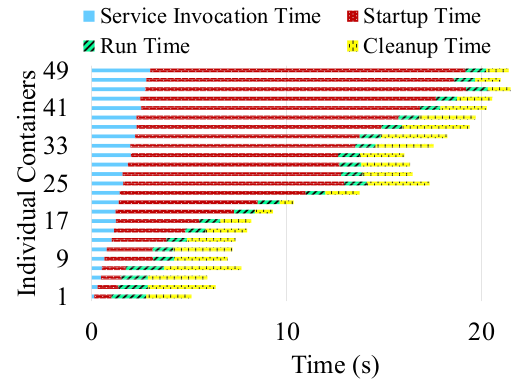
\includegraphics[width=\linewidth]{figs/coldstart-importance}
	\caption {اهمیت شروع‌سرد}
	\label{fig:coldstart-importance}
\end{figure}

\par
ستون قرمز رنگ زمان آماده سازی کانتینر را نمایش می‌دهد. این زمان همان زمان شروع سرد است که دلایل مختلفی از جمله آماده‌سازی کانتینر یا حضور در صف انتظار برای تخصیص منابع باشد. بنابراین، با به‌کارگیری یک استراتژی مناسب می‌توان این زمان را به حداقل رسانید. 

\par 
متاسفانه تاخیر شروع سرد باعث شده تا توسعه‌دهندگان اقبال کمتری به استفاده از پلتفرم‌های بدون سرور داشته باشند. به گونه‌ای که از بین 1000 برنامه‌ی کاربردی بزرگ در پلتفرم \lr{Microsoft Azure}، تنها یک مورد مربوط به یک برنامه تجاری باشد\cite{shahrad2020serverless}. این موضوع  نشان می‌دهد که علی‌رغم پتانسیل بالای رایانش بدون سرور، وجود مشکلات جدی ازجمله شروع سرد، باعث امتناع توسعه‌دهندگان از مهاجرت به پلتفرم‌های بدون سرور باشد. 

\par 
\section{نتیجه‌های مهم تحقیق}
لورم ایپسوم متن ساختگی با تولید سادگی نامفهوم از صنعت چاپ، و با استفاده از طراحان گرافیک است، چاپگرها و متون بلکه روزنامه و مجله در ستون و سطرآنچنان که لازم است، و برای شرایط فعلی تکنولوژی مورد نیاز، و کاربردهای متنوع با هدف بهبود ابزارهای کاربردی می باشد، کتابهای زیادی در شصت و سه درصد گذشته حال و آینده، شناخت فراوان جامعه و متخصصان را می طلبد، تا با نرم افزارها شناخت بیشتری را برای طراحان رایانه ای علی الخصوص طراحان خلاقی، و فرهنگ پیشرو در زبان فارسی ایجاد کرد، در این صورت می توان امید داشت که تمام و دشواری موجود در ارائه راهکارها، و شرایط سخت تایپ به پایان رسد و زمان مورد نیاز شامل حروفچینی دستاوردهای اصلی، و جوابگوی سوالات پیوسته اهل دنیای موجود طراحی اساسا مورد استفاده قرار گیرد.

\par
\par
ساختار این گزارش به این ترتیب خواهد بود:‌

‫در\hyperref[literature] {ادبیات موضوع} مروری بر واژگان، مفاهیم تخصصی و هر آن‌چه که در ادامه به آن نیاز پیدا خواهیم کرد، خواهیم داشت. سپس در فصل
\hyperref[related-works]{کار‌های مرتبط}
  به بیان مشروح تحقیقات انجام شده خواهیم پرداخت و در  
\hyperref[conclusion]{نتیجه‌گیری و کار‌های آینده}
  خلاصه‌ای از مطالعات انجام شده و مسائل باز خواهیم پرداخت. ‬